\documentclass[12pt,a4paper]{article}
\usepackage{hyperref}
\usepackage{float}
\usepackage{graphicx}
\usepackage[utf8]{inputenc}
\usepackage{amsmath}
\usepackage{amsfonts}
\usepackage{amssymb}
\author{Howard Cheung \\ email: howard.at (at) gmail.com }
\title{User manual for the Data Preprocessing Helper Version 0.1}
\begin{document}

\maketitle

\section{Introduction}

This tool is made to assist data analysts who are unfamiliar with coding languages to preprocess their time-series data.
In a lot of engineering systems, data from different subsystems are obtained differently.
While some of them are obtained at different fixed time intervals, some of them, such as on/off signals, are obtained according to time-of-value-change.
The resultant data are very difficult for laymen who only use spreadsheet software to analyze their data.
This project aims at helping these analysts to preprocess their data by converting the time-of-value-change data to data collected at fixed time intervals.

\section{Tutorial}

This tutorial gives a quick tour on how to convert a file with time-of-value-change data to a file at fixed time intervals. First we start with a csv file with the structure in Figure \ref{fig:ugly_file}.

\begin{figure}[H]
\centering
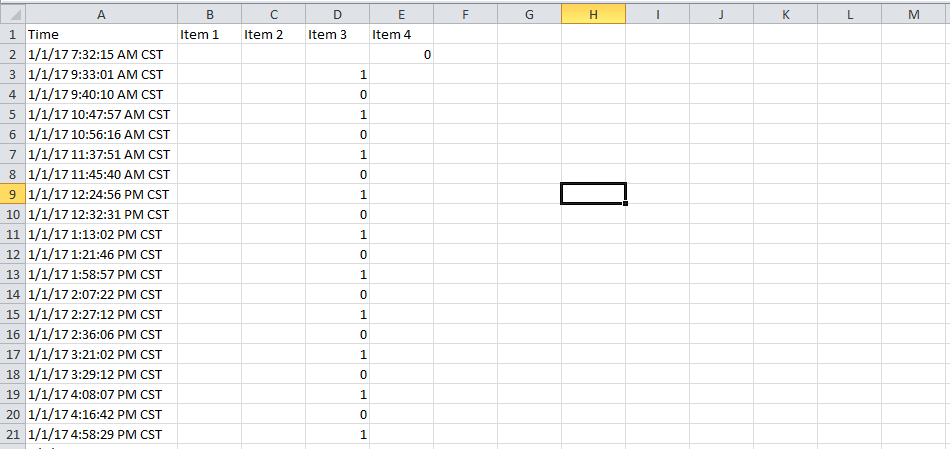
\includegraphics[width=0.8\textwidth]{time-of-change.png}
\caption{Structure of data with time-of-change values}
\label{fig:ugly_file}
\end{figure}

As you can see, there are a lot of unavailable values in Figure \ref{fig:ugly_file}. The timestamps on the left are also ugly because they are all acquired at different time intervals. It is very difficult to try comparing this set of data side-by-side with the other data set.

To convert the data in Figure \ref{fig:ugly_file}, we can use the tool provided in this project. The tool is wrapped as an executable so that you don't have to worry about linking your confidential data to the web to do the filtering. Its user interface is shown in Figure \ref{fig:ui}.

\begin{figure}[H]
\centering
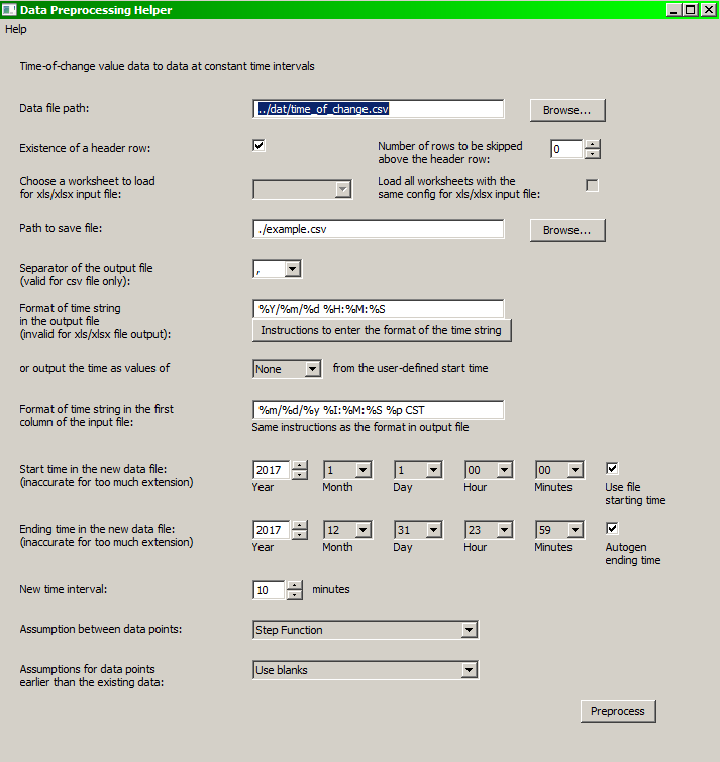
\includegraphics[width=0.6\textwidth]{ui.png}
\caption{Graphical user interface of the tool}
\label{fig:ui}
\end{figure}

To use the tool, use the first "Browse..." button on the right to choose the data file that you want to convert, and click the second "Browse..." button on the right to choose the directory where you want to save your file. Currently, it supports csv file (\href{https://en.wikipedia.org/wiki/Comma-separated_values}{Comma-separated Value File}), xls file (Microsoft Excel 1997-2003 File) and xlsx file (Microsoft Excel Open XML Format File). The locations of the two "Browse..." buttons are shown in Figure \ref{fig:ui_zoomed}.

\begin{figure}[H]
\centering
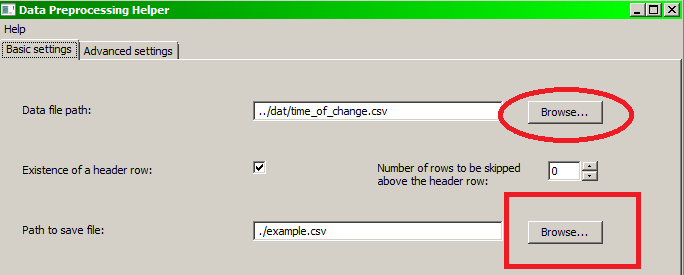
\includegraphics[width=0.6\textwidth]{ui_zoomed.png}
\caption{Location of the first "Browse..." button (in a circle), the second "Browse..." button (in a rectangle) and the text box for entering the format of the time string in the data file (in a pentagon)}
\label{fig:ui_zoomed}
\end{figure}

After that, you need to enter the format of the time string on the leftmost column of your data. The default setting is '\%m/\%d/\%y \%I:\%M:\%S \%p CST' supports a format which looks like

12/31/17 7:32:15 AM CST

. Other typical example of time string is shown in Table \ref{tb:sample_timestring}.

\begin{table}[H]
\caption{Sample format string for different types of time string in the data file}
\begin{tabular}{|p{6cm}|l|}
\hline
Format time string to be entered in the tool & Example time string being support \\ \hline
\%m/\%d/\%y \%I:\%M:\%S \%p CST & 12/31/17 7:32:15 AM CST  \\
 & 1/15/17 11:33:05 PM CST \\ \hline
\%Y/\%m/\%d \%H:\%M:\%S & 2017/12/31 13:00:30  \\
 & 1998/01/32 01:23:02 \\ \hline
 \%y-\%b-\%d \%I:\%M \%p & 99-Jan-01 12:01 AM \\
 & 00-Feb-31 01:08 PM \\ \hline
\end{tabular}
\label{tb:sample_timestring}
\end{table}

Details of their meaning can be found \href{https://docs.python.org/3.5/library/datetime.html\#strftime-and-strptime-behavior}{here}.

After that, all you need is to press the "Preprocess" button on the right hand corner, and you will have your file when the dialog box in Figure \ref{fig:complete} appears.

\begin{figure}[H]
\centering
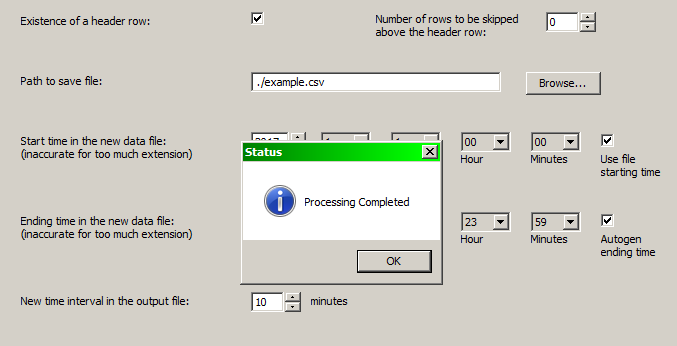
\includegraphics[width=0.6\textwidth]{complete.png}
\caption{Dialog box showing completion}
\label{fig:complete}
\end{figure}

And you can open the file at your selected location as Figure \ref{fig:step}

\begin{figure}[H]
\centering
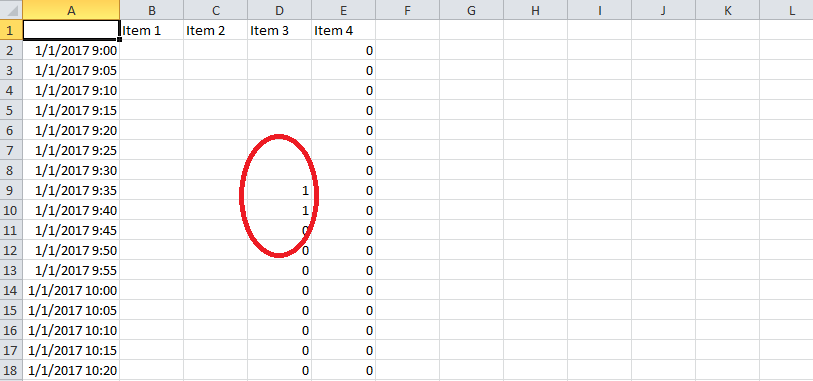
\includegraphics[width=0.6\textwidth]{step.png}
\caption{Dialog box showing completion}
\label{fig:step}
\end{figure}

There are other functions in the tool such as changing the time interval in the output file, using interpolation instead of step function, etc. While they are available for you to explore in this version of tool, their documentation has not been completed. Details of the functions will be discussed in documentation in future versions.

\section{Inquiries}

If you encounter bugs about the tool, please send an email to me at howard.at (at) gmail.com or post an issue at \href{https://github.com/howardcheung/auto-data-preprocessor/}{the GitHub repository}.

\section{License}

Please refer to the website at \href{https://github.com/howardcheung/auto-data-preprocessor/}{the GitHub repository} for the most up-to-date information about the licenses.

\end{document}